%
% This is a borrowed LaTeX template file for lecture notes for CS267,
% Applications of Parallel Computing, UCBerkeley EECS Department.
% Now being used for CMU's 10725 Fall 2012 Optimization course
% taught by Geoff Gordon and Ryan Tibshirani.  When preparing
% LaTeX notes for this class, please use this template.
%
% To familiarize yourself with this template, the body contains
% some examples of its use.  Look them over.  Then you can
% run LaTeX on this file.  After you have LaTeXed this file then
% you can look over the result either by printing it out with
% dvips or using xdvi. "pdflatex template.tex" should also work.
%

\documentclass[twoside]{article}
\setlength{\oddsidemargin}{0.25 in}
\setlength{\evensidemargin}{-0.25 in}
\setlength{\topmargin}{-0.6 in}
\setlength{\textwidth}{6.5 in}
\setlength{\textheight}{8.5 in}
\setlength{\headsep}{0.75 in}
\setlength{\parindent}{0 in}
\setlength{\parskip}{0.1 in}

%
% ADD PACKAGES here:
%

\usepackage{amsmath,amsfonts,graphicx,amsthm,amssymb}
\usepackage{hyperref}
\usepackage[ruled,vlined]{algorithm2e}
\usepackage{cancel}

\hypersetup{
    colorlinks=true,
    linkcolor=blue,
    filecolor=magenta,
    urlcolor=blue,
}

%
% The following commands set up the lecnum (lecture number)
% counter and make various numbering schemes work relative
% to the lecture number.
%
\newcommand*{\QEDB}{\hfill\ensuremath{\square}}%
\newcommand*\xor{\mathbin{\oplus}}
\newcounter{lecnum}
\renewcommand{\thepage}{\thelecnum-\arabic{page}}
\renewcommand{\thesection}{\thelecnum.\arabic{section}}
\renewcommand{\theequation}{\thelecnum.\arabic{equation}}
\renewcommand{\thefigure}{\thelecnum.\arabic{figure}}
\renewcommand{\thetable}{\thelecnum.\arabic{table}}

%
% The following macro is used to generate the header.
%
\newcommand{\lecture}[4]{
   \pagestyle{myheadings}
   \thispagestyle{plain}
   \newpage
   \setcounter{lecnum}{#1}
   \setcounter{page}{1}
   \noindent
   \begin{center}
   \framebox{
      \vbox{\vspace{2mm}
    \hbox to 6.28in { {\bf EE 381V: Special Topics on Unsupervised Learning
        \hfill Spring 2018} }
       \vspace{4mm}
       \hbox to 6.28in { {\Large \hfill Lecture #1: #2  \hfill} }
       \vspace{2mm}
       \hbox to 6.28in { {\it Lecturer: #3 \hfill Scribes: #4} }
      \vspace{2mm}}
   }
   \end{center}
   \markboth{Lecture #1: #2}{Lecture #1: #2}

   % {\bf Note}: {\it LaTeX template courtesy of UC Berkeley EECS dept.}

   % {\bf Disclaimer}: {\it These notes have not been subjected to the
   % usual scrutiny reserved for formal publications.  They may be distributed
   % outside this class only with the permission of the Instructor.}
   \vspace*{4mm}
}
%
% Convention for citations is authors' initials followed by the year.
% For example, to cite a paper by Leighton and Maggs you would type
% \cite{LM89}, and to cite a paper by Strassen you would type \cite{S69}.
% (To avoid bibliography problems, for now we redefine the \cite command.)
% Also commands that create a suitable format for the reference list.
\renewcommand{\cite}[1]{[#1]}
\def\beginrefs{\begin{list}%
        {[\arabic{equation}]}{\usecounter{equation}
         \setlength{\leftmargin}{2.0truecm}\setlength{\labelsep}{0.4truecm}%
         \setlength{\labelwidth}{1.6truecm}}}
\def\endrefs{\end{list}}
\def\bibentry#1{\item[\hbox{[#1]}]}

%Use this command for a figure; it puts a figure in wherever you want it.
%usage: \fig{NUMBER}{SPACE-IN-INCHES}{CAPTION}
\newcommand{\indep}{\rotatebox[origin=c]{90}{$\models$}}
\newcommand{\fig}[3]{
			\vspace{#2}
			\begin{center}
			Figure \thelecnum.#1:~#3
			\end{center}
	}
% Use these for theorems, lemmas, proofs, etc.
\theoremstyle{definition}
\newtheorem{theorem}{Theorem}[lecnum]
\newtheorem{example}[theorem]{Example}
\newtheorem{lemma}[theorem]{Lemma}
\newtheorem{proposition}[theorem]{Proposition}
\newtheorem{claim}[theorem]{Claim}
\newtheorem{corollary}[theorem]{Corollary}
\newtheorem{note}[theorem]{Note}
\newtheorem{definition}[theorem]{Definition}

% **** IF YOU WANT TO DEFINE ADDITIONAL MACROS FOR YOURSELF, PUT THEM HERE:

\newcommand\E{\mathbb{E}}
\newtheorem{problem}{Problem}
\DeclareMathOperator*{\argmax}{arg\,max}
\newenvironment{subproof}[1][\proofname]{%
  \renewcommand{\qedsymbol}{$\blacksquare$}%
  \begin{proof}[#1]%
}{%
  \end{proof}%
}
\allowdisplaybreaks


\begin{document}
%FILL IN THE RIGHT INFO.
%\lecture{**LECTURE-NUMBER**}{**DATE**}{**LECTURER**}{**SCRIBE**}
\lecture{7}{February 8th}{Professor Alex Dimakis}{Justin Lewis, Dany Haddad}
%\footnotetext{These notes are partially based on those of Nigel Mansell.}

% **** YOUR NOTES GO HERE:

% Some general latex examples and examples making use of the
% macros follow.
%**** IN GENERAL, BE BRIEF. LONG SCRIBE NOTES, NO MATTER HOW WELL WRITTEN,
%**** ARE NEVER READ BY ANYBODY.


\subsubsection*{Topics Covered} % Don't be this informal in your notes!
\begin{itemize}
\item Submodularity
\item Feature selection (see \cite{KG05-1})
\item Nemhauser's proof for greedy maximization of submodular functions
\end{itemize}

\section{Definitions}

\subsubsection*{Entropy}
Given a set, $S$, of discrete random variables, define
the set function $f_H(S): 2^\mathcal{X} \mapsto \mathbb{R}$
$$f_H(S) = H(X_S) = - \sum_{x_i \in S} p(x_i)\log p(x_i) $$
and for differential entropy:

$$f_H(S) = H(X_S) = - \int_{\mathcal{X}_S} p(x)\log p(x)dx $$

\subsubsection*{Mutual Information}
Given random vectors $Y$ and $X_S$, define the following as the mutual
information between them $f_I(S):~2^\mathcal{X}~\mapsto~\mathbb{R}$
$$f_I(S) = I(Y; X_S) = H(Y) - H(Y | X_S)$$

\section{Properties}

\begin{lemma}
$f_H$ is submodular.
\end{lemma}

\begin{proof}
  Consider subsets $A$ and $B$ of random variables,
  $\mathcal{X}$, where $A \subseteq B$. Also consider a random
  variable $X_m \notin A \cup B$
  $$f_H(X_A , X_{\{m\}}) - f_H(X_A) = H(X_A, X_m) - H(X_A) = H(X_m | X_A)$$
  \centering and similarly
  $$f_H(X_B , X_{\{m\}}) - f_H(X_B) = H(X_m | X_B)$$
  Since conditioning on a larger set of random variables cannot
  increase the entropy:
  \begin{align*}
    H(X_m | X_B) & \leq H(X_m | X_A) \\
    f_H(X_B , X_{\{m\}}) - f_H(X_B) & \leq f_H(X_A , X_{\{m\}}) - f_H(X_A)
  \end{align*}
\end{proof}

% \begin{note}
%   $2^{H(X)}$ is the volume of the support set of $X$.
% \end{note}

In the discrete case we can show that $f_H$ is also monotone. However,
in the continuous case, this function is no longer
monotone, in general\cite{KG14}.

\begin{example}
  Consider $X_1, ..., X_n$ jointly gaussian random variables with pdf:
  $$p(x) = \frac{1}{\sqrt{2\pi \det \Sigma}} e^{-\frac{1}{2}(x-\mu)^T
    \Sigma^{-1} (x-\mu)}$$

  The differential entropy of a subset indexed by $S$ is given by:
  $$H(X_S) = \frac{1}{2} 2 \pi e\log \det \Sigma_s$$
  Where $\Sigma_S$ denotes the submatrix of the covariance matrix
  $\Sigma$ formed by taking only the variables indexed by $S$.

  Consider the covariance matrix:

  \begin{align}
    \Sigma =
    \begin{bmatrix}
               1 & 0 & 0 & 0 \\
               0 & 2 & 0 & 0 \\
               0 & 0 & 0.1 & 0 \\
               0 & 0 & 0 & 3  \notag
             \end{bmatrix}
  \end{align}

  \begin{align*}
    & \det(\Sigma_{\{0\}}) = 1\\
    & \det(\Sigma_{\{0, 1\}}) = 2\\
    & \det(\Sigma_{\{0, 1, 2\}}) = 0.2\\
    & \det(\Sigma_{\{0, 1, 2, 3\}}) = 0.6
  \end{align*}
  So $H(X_\mathcal{X})$ is not monotone in this case.
  \QEDB
\end{example}

\begin{note}
  In the above example, to choose the subset of $k$ variables with the
  largest entropy, we must maximize the determinant of $\Sigma_S$.
\end{note}

\begin{proposition}
  Mutual information is, in general, not submodular.
\end{proposition}
\begin{proof}
  Recall the set function for mutual information as defined earlier, $f_I(S) = I(Y; X_S)$

  Consider $X_1$, $X_2$
  independent $Bernoulli(\frac{1}{2})$ random variables. Let $Y = X_1
  \xor X_2$. So:
  \begin{align*}
    H(Y) &= H (Y | X_1) = H (Y | X_2) = 1  \text{ and } H (Y | X_1,
           X_2) = 0 \\
         & \implies H(Y) - H(Y | X_1) \leq H (Y) - H (Y | X_1, X_2) \\
         & \implies f_I(\{1\} | \emptyset) < f_I(\{1\} | \{2\})
  \end{align*}
\end{proof}

\begin{claim}
  Mutual information is monotone. This follows immediately from
  the fact that conditioning does not increase entropy.
\end{claim}

\begin{proposition}
  Given sets $S$ and $U$ of random variables such that the elements of
  $S$ are independent of each other conditioned on $U$, then $f_I(A) = I(U;
  A)$
  is submodular for all $A \subseteq S \cup U$.
\end{proposition}

\begin{proof}
  Let $A \subseteq S \cup U$ and $S_1 \indep S_2$ conditioned on
  $U$ $ \forall S_1, S_2 \subseteq S$.
  \begin{align} \label{eq:1}
    I(U; A) &= H(U) - H(U | A) \nonumber\\
            &= H(U) - (H(U \cup A) - H(A)) \nonumber\\
            &= H(U) - (H(A | U) + H(U) - H(A)) \nonumber\\
            &= -\sum_{y \in A \cap S} H(y | U) + H(A)
  \end{align}
  Where the last step follows by conditional independence the elements
  of $S$ conditioned on $U$. The first term in equation \ref{eq:1} is
  modular in $A$ and the second is submodular.
\end{proof}

\begin{figure}[h]
  \centering
  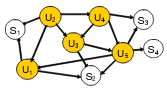
\includegraphics[scale=0.8]{cond_ind.png}
  \caption{An directed graphical model where the elemets of $S$ are
    independent conditioned on $U$}
  \label{fig:ugm}
\end{figure}

This claim holds if the distribution factorizes according to a
graphical model similar to \ref{fig:ugm}. Recall the conditional
independence properties we can infer from directed and undirected graphical
models.

\section{Optimization}
The sensor selection problem addressed in \cite{KG05-1} is framed as
a joint entropy maximization problem. Intuitively, we can think of this
problem equivalently as minimizing the uncertainty of the sensors that
are not selected (since they will not be observed). One might suggest
a PCA type solution to this problem, but unfortunately, these are
physical sensors that we are selecting, so we cannot take a linear
combination of them! Gram-–Schmidt will not save you here!

Consider the chain rule of entropy:
$$H(X_1, ..., X_n) = H(X_S) + H(X_{S^c} | X_S)$$
Since $H(X_1, ..., X_n)$ has no dependence on $S$, maximizing the
entropy of the subset $S$, is equivalent to minimizing the
uncertainty of the unobserved set, $S^c$:
$$\max_{s: |s| \leq k} H(X_S) = \min_{s: |s| \leq k} H(X_{S^c} |
X_S)$$
This requires us to maximize a monotone submodular function. The
greedy algorithm selects the element with the largest discrete
derivative at iteration $i$.


%----------------------------------------------------------------------------------------
%----------------------------------------------------------------------------------------
\newpage
\section{Approx. Submodular Function Maximization}


It is well known that maximizing an arbitrary submodular function with
given constraint set is, in general, NP-Hard. %(REFERENCE?)

\begin{problem}
Given ground set $S_g$, subset $S \subseteq S_g$, and submodular set function $f(\cdot)$:

\begin{equation*}
  \begin{split}
    \max_{S \, \subseteq \, S_g} &f(S)\\
    \text{subject to } &|S| \leq k
  \end{split}
\end{equation*}

\end{problem}

%To reiterate, there are a number of well known problems which reduce to submodular maximization (UNNECESSARY?):
%
%\begin{itemize}
%\item Max cut
%\item Max cover
%\item Sensor selection
%\item Knapsack problem
%\end{itemize}

\newcommand{\spbigvert}{\, \big \vert \,}
\newcommand{\spvert}{\, \vert \,}

Finding the optimal solution may be intractable; however, an approximate solution known as the Greedy Algorithm can achieve fair results. More specifically:

\begin{algorithm}[H]
\SetAlgoLined
\caption{Greedy Algorithm}
\SetKw{Kw}{Define}
\Kw{ground set $S_g$, subset $S \subseteq S_g$, set function $f(\cdot)$, and cardinality constraint $|S| \leq k$  }\;
\SetKw{Kw}{Description}
\Kw{ greedily add to $S$ at iteration $i$ the element with the largest discrete derivative}\;
\KwResult{$S_{greedy}$ }
 $S_0=\emptyset$\;
 $i=0$\;
 \While{$|S_{i}| \leq k-1$}{
  $\displaystyle S_{i+1} = S_i \, \cup \, \argmax_{s \in \{S_g \setminus S_i\}} \bigg\{ \Delta_f(s \spvert S_i) \bigg\}$ \;
  $i=i+1$\;
 }
\SetKw{Kw}{Return}
\Kw{$S_{i+1}$}\;
\end{algorithm}

\underline{Recall:} For set function $f: 2^V \rightarrow \mathbb{R}, S \subseteq V,$
and $e \in V$ \\
let $\Delta_f(e \spvert S) := f(S \cup \{e\}) - f(S)$



\begin{theorem}
Let $S^*$ denote the optimal subset , and $S_{greedy,\ell}$ as the Greedy Algorithm selection after $\ell$ iterations. Given set function $f$ which is submodular, monotone, non-negative, and $f(\emptyset)=0$ :

$f(S_{greedy,\ell}) \geq [1-\text{exp}[-\dfrac{\ell}{k}]] \cdot f(S^*)$
	
$f(S_{greedy,\ell=k}) \geq [1-\dfrac{1}{e}] \cdot f(S^*) \approx 0.63 \cdot f(S^*)$

\end{theorem}

\begin{proof}
  \cite{NW78}


Let $S_i$ denote the Greedy algorithm selection after the $i$-th iteration

$f(S^*) \leq f(S^* \cup S_i)$ $\text{(monotonicity)}$

\newpage
\begin{claim}
$\displaystyle f(S^* \cup S_i) = f(S_i) + \sum_{j=1}^{k} \Delta_f \bigg(v_j^* \spbigvert \big\{S_i \cup \{v_1^*,v_2^*,\ldots,v_{j-1}^*\}\big\}\bigg)$

\begin{subproof}[Subproof]
Expand:
%%%%
\begin{flalign*}
\displaystyle f(S^* \cup S_i) &= f(S_i) + \Delta_f \big(v_1^* \spbigvert S_i \big)
+\Delta_f \bigg(v_2^* \spbigvert \big\{S_i \cup v_1^*\big\}\bigg)
+\cdots 
+\Delta_f \bigg(v_k^* \spbigvert\big\{S_i \cup \{v_1^*,v_2^*,\ldots,v_{k-1}^*\}\big\}\bigg) &\\
%%%%
&= \cancel{f(S_i)} + \cancel{{f(S_i \cup v_1^*)}} - \cancel{{f(S_i)}}
+ \cdots + f(S_i \cup \{v_1^*,v_2^*,\ldots,v_{k}^*\}) 
-\cancel{f(S_i \cup \{v_1^*,v_2^*,\ldots,v_{k-1}^*\})}  &\\
%%%%
&= f(S^* \cup S_i)
\end{flalign*}

The telescoping sum leaves only the desired term.

\end{subproof}
\end{claim}
%%%%
With claim above it follows: %%REFERENCE step 1?
%%%%
\begin{flalign*}
f(S^*) \leq f(S^* \cup S_i) &=  f(S_i) + \sum_{j=1}^{k} \Delta_f \bigg(v_j^* \spbigvert \big\{S_i \cup \{v_1^*,v_2^*,\ldots,v_{j-1}^*\}\big\}\bigg) & &\\
&\leq f(S_i) + \sum_{j=1}^{k} \Delta_f (v_j^* \spbigvert S_i) &\text{(by submodularity)} &\\
&\leq f(S_i) + \sum_{j=1}^{k} [f(S_{i+1})-f(S_i)] & \text{(by Greedy selection)} &\\
&= f(S_i) +k\cdot[f(S_{i+1})-f(S_i)]&\\
&\\
\Rightarrow f(S^*)-f(S_i) &\leq k\cdot[f(S_{i+1})-f(S_i)] &\\
\delta_i &\leq k\cdot[\delta_i-\delta_{i+1}] &(\delta_i \triangleq f(S^*)-f(S_i)) &\\
\delta_{i+1} &\leq (1-\dfrac{1}{k})\cdot\delta_i &\\
\delta_\ell &\leq (1-\dfrac{1}{k})^\ell\cdot\delta_0 &\\
&\\
f(S_\ell) &\geq (1-(1-\dfrac{1}{k})^\ell)\cdot f(S^*) 
&(\delta_0 = f(S^*)-f(\emptyset)=f(S^*) &\\
f(S_\ell) &\geq (1-\text{exp}(-\dfrac{\ell}{k}))\cdot f(S^*)
&(1-x \leq \text{e}^{-x} \,\, \forall \, x) &\\
\end{flalign*}
\end{proof}

\newpage

\section{Next Time: Feature Selection}

The feature selection problem given by:
\begin{equation*}
  \begin{split}
    \max_{\beta} &||X\beta - y||_2^2\\
    \text{subject to } & ||\beta||_0 \leq k
  \end{split}
\end{equation*}
can be relaxed by changing the $\ell_0$ norm for an $\ell_1$
norm. Bringing the constraint into the objective and setting $\lambda$
as a hyperparameter, we arrive at the LASSO problem:

\begin{equation*}
  \begin{split}
    \max_{\beta} &||X\beta - y||_2^2 + \lambda ||\beta||_1\\
  \end{split}
\end{equation*}

Alternatively, we can frame the objective as a set function
$f(S) = ||X_S\beta_S||_2^2$ and show that if the columns of $X$ are
orthogonal, then $f$ is submodular. Otherwise, $f$ is weakly submodular
if $X$ satisfies the restricted isometry property (RIP).

\newpage
\section*{References}
\beginrefs
\bibentry{KG05-1}{\sc Krause, Andreas and Guestrin, Carlos},
``Near-optimal sensor placements,''
{\it Proceedings of the fifth international conference on Information
  processing in sensor networks - IPSN 06}, 2005.

\bibentry{KG05-2}{\sc Krause, Andreas and Guestrin, Carlos},
``Near-optimal Nonmyopic Value of Information in Graphical Models,''
{\it Proceedings of the Twenty-First Conference on Uncertainty in
  Artificial Intelligence}, 2005.

\bibentry{KG14}{\sc Krause, Andreas, and Daniel Golovin},
``Submodular function maximization,'' 2014.

\bibentry{NW78}{\sc Nemhauser, George L., Laurence A. Wolsey, and Marshall L. Fisher},
``An analysis of approximations for maximizing submodular set functions,''
{\it Mathematical Programming}, 1978.
\endrefs

% **** THIS ENDS THE EXAMPLES. DON'T DELETE THE FOLLOWING LINE:

\end{document}
